\section{Simulation of HCCP and LEACH}
\label{ch:sim}


A custom simulator was developed to simulate the running of HCCP. Other network simulation suites
are available, such as OmNet++~\cite{omnet} with its related suites such as Castalia~\cite{castalia}  are
widely used, and provide tools for analysis. These tools were tested, and were deemed unfit for the 
desired simulation setups. Tracking the number of messages sent, from where, route taken and 
number of times a given message has been received at the sink are possible, but difficult to collect.
OmNet++ messages can only be in one mote's message queue at a time since it can only have one `owner'.
Since a message can only have one owner, it is very difficult to track how many times a given 
message has been received at the sink. Also, the MAC layer protocol is not simple to change while
running a simulation. LEACH uses both CSMA and TDMA MAC protocols, so to properly simulate LEACH either 
switching the MAC protocol must occur, or the finer details of the protocols must be abstracted and be viewed simply as access to a radio. 


WSN code can be written 
in such a way that the physical layer can be largely ignored. 
The physical layer controls the  radio, modulating the 
frequency to communicate with surrounding motes. This includes
what frequency or protocol (such as 802.15.4 or ANT radios) the motes use.
The simulator abstracts the physical layer, as it is not the focus of the
simulation or research. 
It is assumed that the radios work, have a given range and draw 
power when on.

When building the simulator, the problem of simulating a WSN was viewed as 
a queuing theory problem more than a networking problem. In doing this, many of 
the network problems are abstracted away, such as radio channels or how collisions can be 
recovered from. HCCP currently only uses one radio channel, so only one channel was
created. Messages that have collided are assumed lost, and unrecoverable.

With these assumptions and abstractions, a simple to understand simulation could be made 
to collect important statistics about the inner workings of the network.



\subsubsection{Simulator Capabilities}
The custom simulator is able to create networks of any size with a two dimensional rectangular space in which
to place the motes. Attention was given to the use of random number generators and 
randomly created events. Random seeds are kept, and random events can happen at the 
same times in networks that are being compared. 

Each mote is given its own random number generator with its own seed to generate random events. 
Separate random number generators are used to draw random numbers for all tasks, ensuring
the simulated motes generate the same random numbers for both the LEACH and HCCP simulations.

The package used to generate random numbers, and to maintain the event queue was SSJ~\cite{SSJ}. 
SSJ is a well-respected Java simulation package. The pseudorandom number generator and the
event queue were built for simulating queuing theory events, and therefore were easily applied to simulating
events in wireless sensor networks.

SSJ provides excellent facilities for collecting statistics on the motes. SSJ can collect continuous 
data, such as calculating what percentage of the time a given mote was on or off; or, collect discrete
events, such as number of messages received, sent and lost.


\subsubsection{Design of Motes in the Simulation}

The custom simulator simulates motes that are an abstraction of motes in real life.
Motes have been abstracted to have the following features:
\begin{enumerate}
	\item \textbf{A battery}: The battery drains faster when the mote is on, and slowly when the mote is sleeping. 
	Motes can draw more power if they are power intensive motes, or less power if they are power efficient motes.
	The batteries can start with more or less energy, which simulates having a larger or smaller battery. Since batteries in
	reality do not always have the same amount of battery power, the 
	simulator applies jitter to the amount of power given to the motes. This amount is configurable, and generally
	assumed to be quite small.
	\item \textbf{A message queue}: The queues contain messages created by this mote, and messages that have hopped into this mote. The 
	queue has finite space. If the queue is full, the message that should be added to the queue is lost.
	\item \textbf{Sensor readings}: Sensor readings happen at a specified frequency. Sensor readings get turned into 
	messages which are added to the message queue. If the message queue is full, the message with the reading is 
	lost.
	\item \textbf{A simple MAC layer}: The MAC layer is designed to be simple and abstract. CSMA uses backoffs of the
	channel is currently being used. CSMA waits a random amount of time before attempting to send the message again. 
	Each mote needs its own random number generator to generate a random backoff time.
	\item \textbf{A radio}: All devices have radios that have a given range. If a neighbouring mote is within range of 
	a device, the two motes can communicate. All radio links are assumed to be one-way links, as some radios
	could have more transmission power than other radios. The units of the range are arbitrary distance units, 
	and could be interpreted as centimetres, metres or even miles.
	\item \textbf{A position}: Motes are given a position on the two dimensional plane. Any mote can be set to 
	be mobile in the network, and can move at any time. This movement will change which surrounding 
	motes the moving mote can communicate with.
\end{enumerate}
This is consistent with the high-level description Akyildiz et al.~\cite{wsnSurvey} gave
to describe a mote, and with Figure~\ref{fig:images_intro_mote}.

Motes can be of various different types: basestations, routing nodes, or sensor nodes. Basestations
are the sinks, once a message is received at the basestation it is marked as completed.  Routing nodes
are motes that have no sensors, and are therefore ideal  for routing messages. Sensor nodes are
motes that make sensor readings, and the sensor readings are turned into messages. The type
of sensors and number of sensors have been abstracted away. Basestations are assumed to have wall power, sensor and routing 
nodes are generally assumed to have battery power, but the simulator has the capabilities of giving them wall power.

Heterogeneity is given to the motes by initializing the motes with different properties, such as:
\begin{itemize} 
	\item more or less battery power 
	\item more or less power drawn when on or off 
	\item more or less available space for a message queue
	\item longer or shorter radio transmission range
	\item the ability to move or not and how fast the movement is
	\item frequency of sensing and creating messages
\end{itemize}

The number of sensors or type of sensors can be abstracted to being a frequency of sensing events. If a mote has many sensors, 
it can be abstracted to have more sensing events. A routing mote is the other extreme, in that a routing mote has 
no sensing events and therefore no frequency of sensing events.

All motes in the custom simulation use common code for the MAC layer, as this is a requirement for heterogeneous WSN. Motes in heterogeneous
WSNs have differing hardware, energy levels and capabilities, but share a common mode of communication.

\paragraph{Motes in the Simulations}

A set of motes were reused for consistency across all the simulations. This provides 
standardization of the motes across the simulations while providing heterogeneity across
the simulations. The power draw of all the motes were kept the same across all the types of motes
for all simulations. The motes varied in queue size and battery size.

\begin{itemize}
    \item \textbf{Router} - A special type of mote that does not have any sensors. It is given a large queue and a large battery making it ideal for routing messages.
    \item \textbf{Normal} - An average mote. Most of the motes in the network are set to this kind of mote. It has an average battery, and an average queue.
    \item \textbf{Expensive} - The expensive mote simulates a mote that has expensive sensors that are power hungry devices. This mote has a larger message queue than the normal mote, but a smaller battery.
    \item \textbf{Very Expensive} - The very expensive mote simulates a mote that has more power hungry sensors than the Expensive mote,  a smaller battery, and a smaller message queue.
    \item \textbf{Super Expensive} - The Super Expensive mote simulates a mote that has the most expensive sensors that put a very large load on the battery. It therefore has the smallest battery, and the smallest message queue.
\end{itemize}

\subsection{Modifications to LEACH for Simulation}
LEACH does not specify which routing algorithms should be used when using LEACH.
For comparison reasons, two routing algorithms were used in creating LEACH: beacon routing 
and 
preset routing, where every node knows its beacon rank from the beginning of the simulation.

In the beacon routing implementation, the mote published its beacon rank when it announced 
it was a clusterhead, during the clusterhead announcement phase. This is not very efficient, but is
a realistic way
of disseminating the routing information to the network.

Since HCCP has facilities to efficiently disseminate routing information, a preset routing simulation was created. The
preset routing simulation sets each of the motes appropriate beacon rank before the simulation starts. This permits the network to work
as if the network has been alive for long enough that the routing information has been disseminated thoughout the network.


\subsection{Modifications to HCCP for Simulation}
HCCP has facilities for routing, but does not specify which routing algorithm should be used. 
Because a routing algorithm is needed for the network to work once it is deployed, the simulation has 
been implemented with beacon routing with HCCP, as HCCP will then be evenly comparable to LEACH. 
The beacon information is disseminated during the roundtable
discussion, as prescribed by HCCP.

Since LEACH has been provided preset routing, the HCCP simulation has also been 
given preset routing, so it can be fairly compared to LEACH. Simulations with
the preset routing tables were done, as were simulations without preset routing tables 
to show the differences in data dissemination between the networks.

% NOTE TO SELF: fake routing is pre-filling the routing tables - CALL IT preset routing



\subsection{Observations and Results}


The worst-case baseline runtime for a mote in the simulation setup is 40,776s (the mote is always on), and the best-case runtime is
256,200s (the mote is only on during the mandatory times). Clearly the best-case is impossible to reach, as all motes would be sleeping 
for the entire cluster runtime (TDMA schedule runtime), never sending any data messages. 
Since the motes are asleep for the entire cluster runtime,  it will also will
never send hop messages, which means the mote will never have its messages reach the sink and is therefore useless. If 
a mote is always a clusterhead, it will be on for the entire simulation making the worst-case runtime a possibility in 
the simulation. Duty-cycling ensures that a mote will never only run as a clusterhead.
% onDraw					1.5
% update 		60
%  500 * 400 
%  81 * 600 avg battery = 427
%  427/1.5
% 427*0.1
% 5 / 5.55
%= 0.9009009009009
%0.55 / 5.55
%= 0.0990990990991
%17080 * 0.9009009009009 + 256200 * 0.0990990990991
%= 40776.5765765768
%
% 
% 



All permutations of the possible Goodness Delay factor configurations were run to provide insight to which 
HCCP parameters that build the Goodness Delay  (described in section~\ref{subsec:goodnessDelay}). 
The permutations were run as the following: 100\% Battery power; 99\% Battery power, 1\% Message queue; 99\% Battery power,
1\% Random; and so on.
Each parameter contributes a percentage of the time that the mote waits before it 
announces its Clusterhead Candidacy or Clusterhead Announcement. Since there are 5 factors,
each are considered separately. The LEACH-style clusterhead percentage is controlled separately from the 
5 HCCP factors and are also viewed separately. Motes will elect to be a Clusterhead Candidate using the same
equation as LEACH uses for electing clusterheads.

The $x$-axis of the following graphs show the percentage that the listed HCCP factor contributes to the
Goodness Delay. The remainder of the Goodness Delay is a permutation of the remaining HCCP factors. For instance:
if the contribution to the Goodness Delay of Battery Power is 50\%, the other 50\% will be made of up all the 
possible permutations of Random, Duty Cycle, Message Queue and Sensor Mission. 
The charts all have the same $x$ and $y$ axis to make comparisons clearer. 


\begin{figure}[htb]
	\centering
		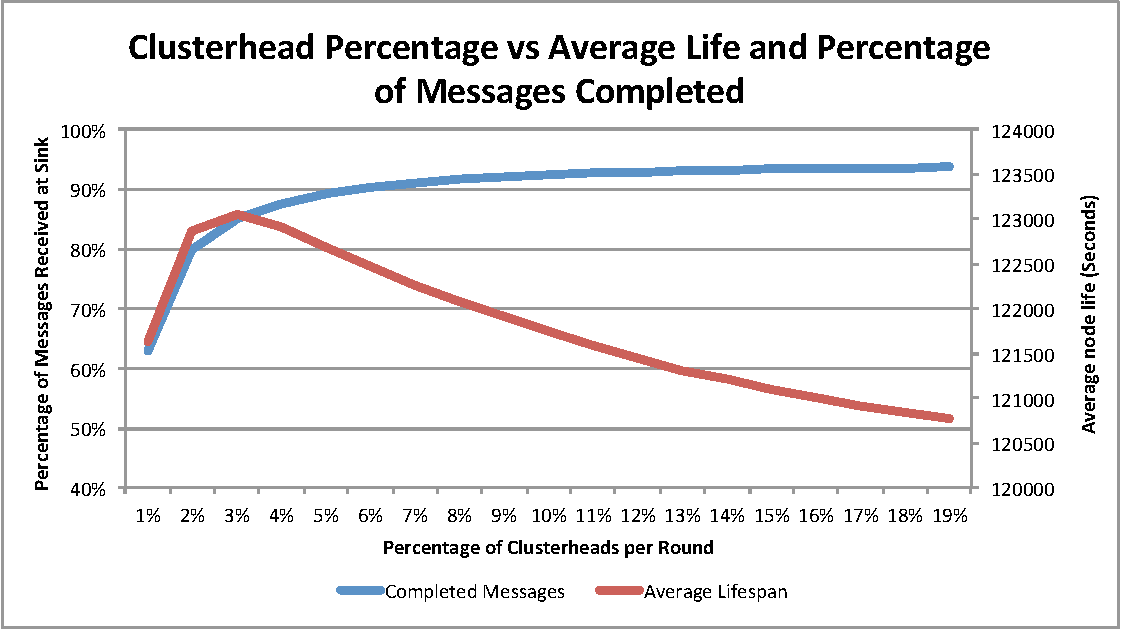
\includegraphics[width=6in]{images/simulation/goodness/clusterhead.pdf}
	\caption{Visualization showing the relationship between Percentage of Clusterheads per round and simulation results.}
	\label{fig:images_simulation_goodness_clusterhead}
\end{figure}


HCCP, much like LEACH, can be set up to vary the percentage of clusterheads per round in the network.
Since motes that are clusterheads use more power per round than motes that are not clusterheads, choosing
a higher percentage of clusterheads per round causes the network to have a shorter lifespan. This effect can 
be seen in Figure~\ref{fig:images_simulation_goodness_clusterhead}, as the percentage of clusterheads increases the 
lifespan of individual motes drops. There is a peak at 3\% clusterheads for average lifespan since motes that choose clusters
turn off for the remainder of the HCCP phase. These small energy savings add up to make the average lifespan of the network 
longer. Heinzelman et al.\cite{leach} also saw the same phenomenon happen while testing LEACH, finding that the motes
dissipate the least energy in their test case at about 5\% clusterheads per round. Since HCCP uses many of
the design elements of LEACH it is not surprising that the two have similar optimal percentages of clusterheads
per round. 

The message throughput increases with the percentage of motes that are clusterheads each round. This makes sense,
as the non-clusterhead motes would have a good selection of clusterheads to choose from, and could choose a
clusterhead that is nearby to decrease the chances of a message collision. However, as the percentage of clusterheads
increases, the lifespan of the network decreases. This causes a tradeoff for a network administrator to choose from, 
as some networks might require longer lifespans, while other networks may value message throughput.

\subsubsection{Effect of Goodness Delay on HCCP}

\begin{figure}[htbp]
    \centering
        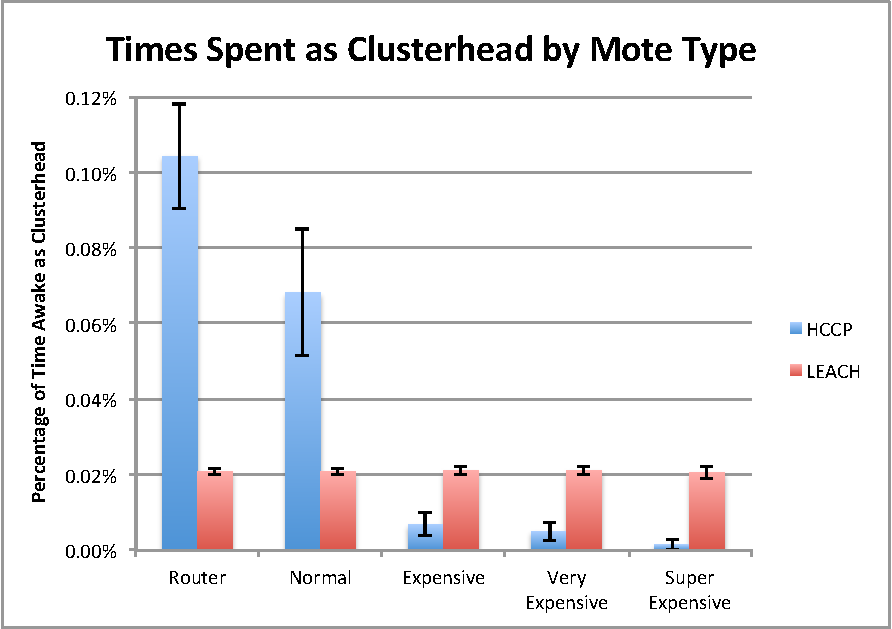
\includegraphics[height=3in]{images/clusterheadChoice/SensorMissionCHTime.pdf}
        % from charts/sensorSmall/nodedata.xlsx
    \caption{The Goodness Delay focuses the clusterhead task on motes that are suited for the task.}
    \label{fig:images_clusterheadChoice_SensorMissionCHTime}
\end{figure}

The Goodness Delay in HCCP is intended to make motes that are well-suited for the task
clusterheads more often. Figure~\ref{fig:images_clusterheadChoice_SensorMissionCHTime} shows
that the Goodness Delay is effective in doing this. As the motes get more expensive, hypothetically
with more power-hungry sensors, the mote gets chosen to be a clusterhead less frequently. This means that 
the mote will draw less power, since it is not being a clusterhead as frequently. 

Note that in Figure~\ref{fig:images_clusterheadChoice_SensorMissionCHTime} the percentages are quite low, as
the the Y axis is the percentage of time  the mote was a clusterhead over the entire
time it was alive, which includes long sleep periods between cycles of the protocol.



\subsection{Discovering how Heterogeneous Factors Effect the Network}
Simulations were run with all the possible permutations of
the factors available in the simulation. The results show which heterogeneous
factors are valuable for improving the WSN. The factors that could be used in 
clusterhead elections in HCCP are: residual battery power, 
available message queue size, sensor mission, when the last time this node was a 
clusterhead was, and a random variable. Breaking the problem down to the separate factors, 
the value of the factors can be compared.


All the permutations of the HCCP factors for Goodness Delay were run on the same network
with the same random seeds. This set up the network with the same starting and running parameters so
that events would happen at the same times in the various networks, allowing the networks 
be comparable 
with the given parameters.

\subsubsection{Effect of Available Queue Size on HCCP Goodness Delay}


Focusing on available queue size for a method of describing how good a mote would do as a clusterhead
is an obvious choice, as clusterheads will be collecting messages from the surrounding motes and need the 
ability to store all the messages. If the message queue is full on a mote, it could not store the new incoming messages, therefore
losing all incoming messages. If incoming messages are lost it not only is negative to the network in terms of information loss,
 but also wastes the energy of the poorly chosen clusterhead and all the motes that register with that cluster.

 \begin{figure}[bthp]
 	\centering
 		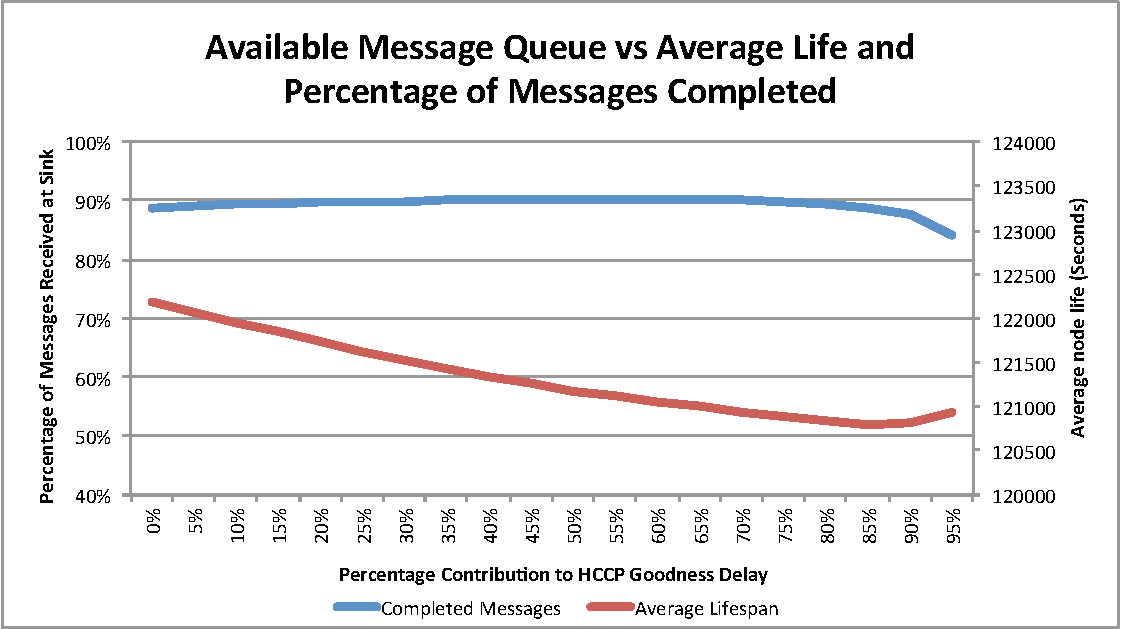
\includegraphics[width=0.9\textwidth]{images/simulation/goodness/AvailableQ3.pdf}
 	\caption{The relationship between HCCP Goodness Delay using Available Queue size and simulation results.}
 	\label{fig:images_simulation_goodness_AvailableQ}
 \end{figure}


The effects of focusing on Message Queue size can be seen in Figure~\ref{fig:images_simulation_goodness_AvailableQ}. 
As the focus on message queue increases, the average lifespan of the network drops. This is not surprising as the focus
on battery power and duty-cycling reduces, making the network solely focus on choosing clusterheads that have
large available message queue size regardless of available power. Because of this, Message Queue size is likely a good 
secondary factor that would control less of the Goodness Delay, balancing a factor such as Battery Power.

% charts/10-1000freqtest
\begin{figure}[htbp]
    \centering
        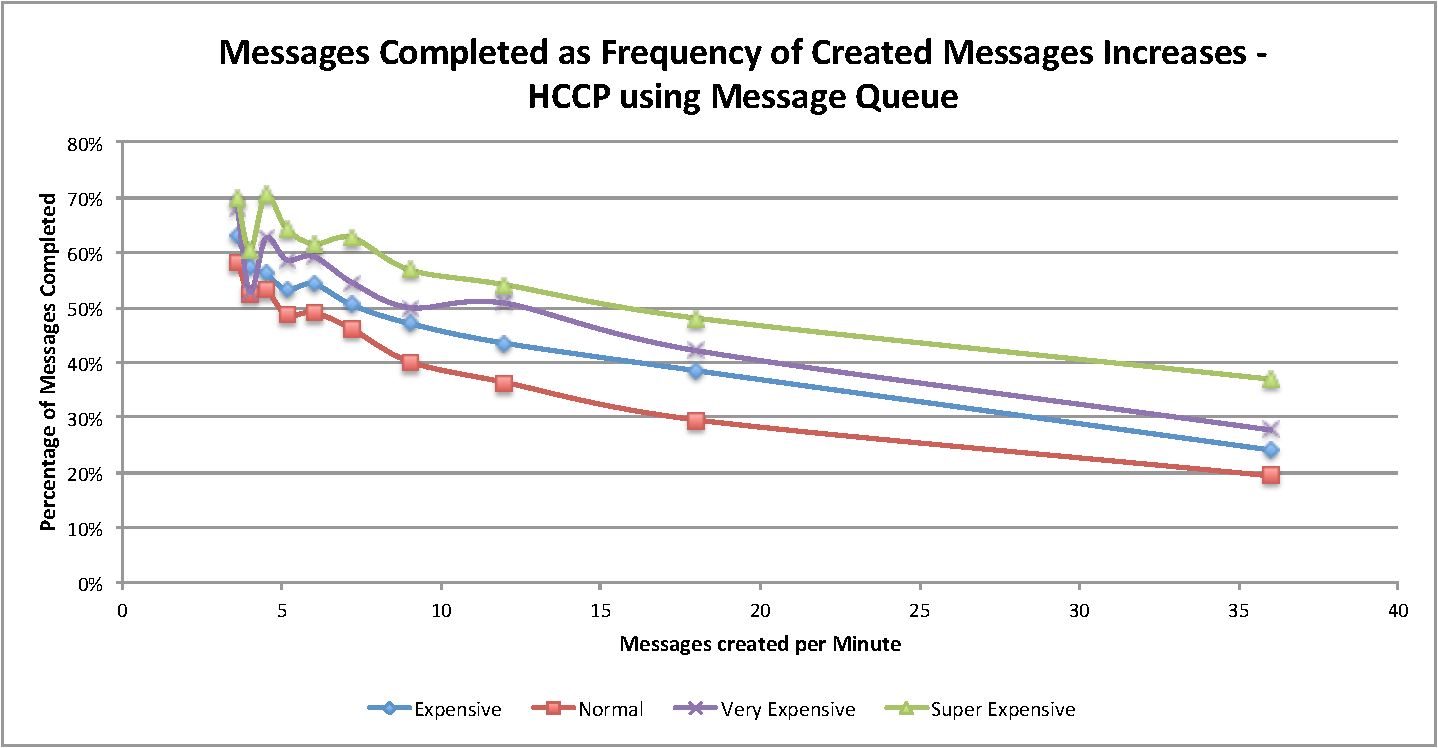
\includegraphics[height=3in]{images/messageFrequency/HCCP.pdf}
    \caption{HCCP handles being overloaded with messages well, as motes with larger available message queues will opt to be clusterheads.}
    \label{fig:images_messageFrequency_HCCP}
\end{figure}

\begin{figure}[htbp]
    \centering
        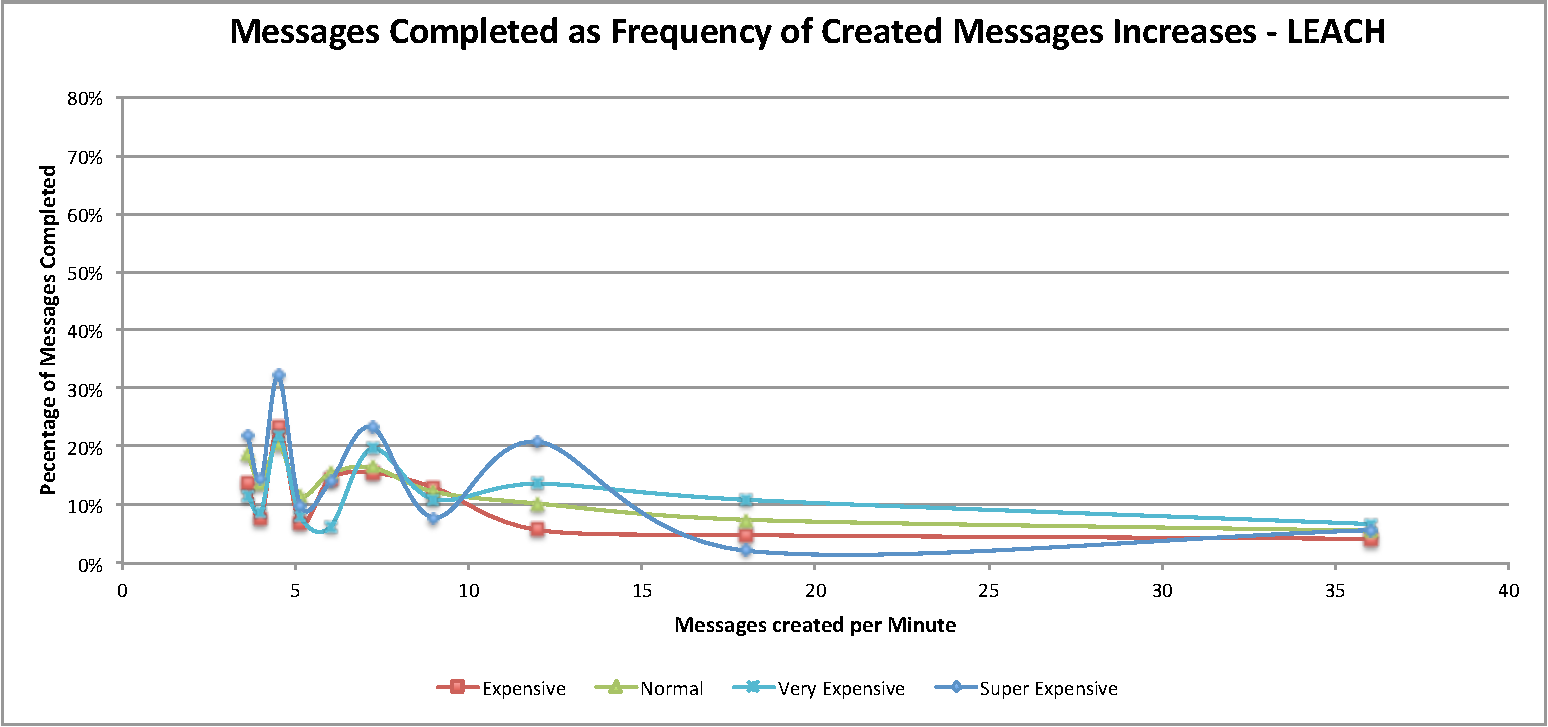
\includegraphics[height=3in]{images/messageFrequency/LEACH.pdf}
    \caption{LEACH does not handle being overloaded, as it does not consider message queue size when electing clusterheads. Note the $y$ axis is the same as Figure~\ref{fig:images_messageFrequency_HCCP}.}
    \label{fig:images_messageFrequency_LEACH}
\end{figure}

As the network gets busier, the chances of any mote having a full message queue is greater. When message queues
start filling up, the importance of focusing on message queue size as a HCCP Goodness Delay factor increases. 
Because HCCP can focus on which motes can be effective clusterheads, better clusterheads will be elected.
The results of this can be seen in Figures~\ref{fig:images_messageFrequency_HCCP} and~\ref{fig:images_messageFrequency_LEACH}, which 
have the same $x$ and $y$ axes to show the difference between the two results.
HCCP can handle a network that is overloaded with messages quite well, because motes with more
available space to hold incoming messages from the clustermotes will be more likely to be clusterheads.

The standard deviation of the simulation is approximately $\pm$20\% for both HCCP and LEACH for each
frequency level. This shows that HCCP focusing on Message Queue has a significant gain over LEACH
in terms of message throughput for Super Expensive motes even at the most overloaded network run. It is 
also interesting to note that the signal-to-noise ratio for LEACH is approximately 100\%, even 
at the least overloaded simulation run.


\begin{figure}[htbp]
    \centering
        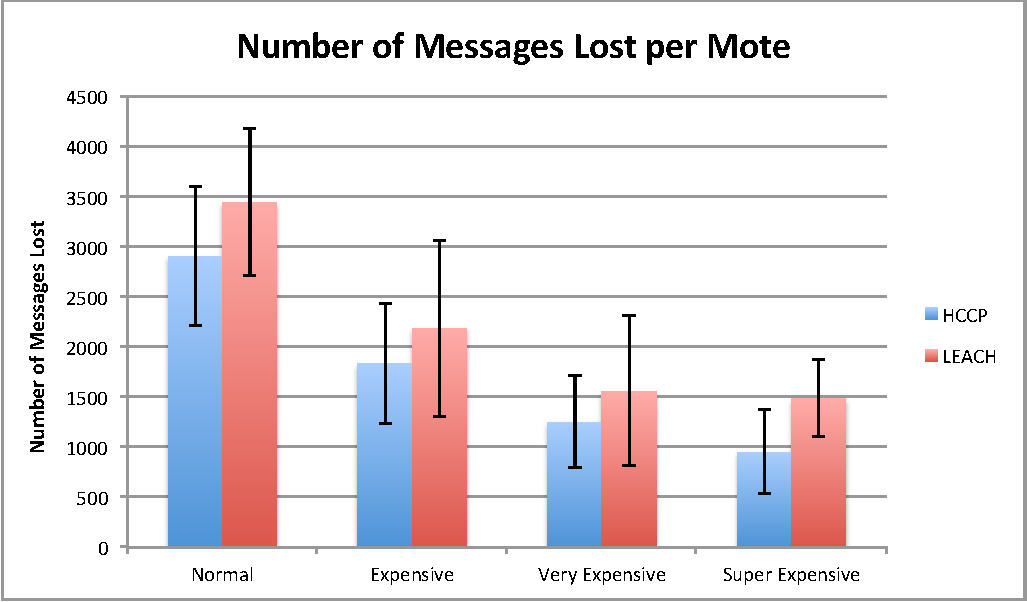
\includegraphics[height=3in]{images/messageFrequency/MessagesLost.pdf}
    \caption{HCCP loses fewer messages due to full message queues than LEACH.}
    \label{fig:images_messageFrequency_MessagesLost}
\end{figure}

HCCP focusing on Message Queue will have the effect that fewer messages 
will be lost due to having no available space in the message queue.
Fewer messages will be lost as motes that have more available message queue space will opt
to be clusterheads, which will then free up space in the surrounding motes to use.
Figure~\ref{fig:images_messageFrequency_MessagesLost} shows that HCCP does 
have fewer lost messages, significantly more for Super Expensive motes. 
This shows that HCCP has gains over LEACH in how many messages are lost due to 
full message queues.

\subsubsection{Effect of Available Battery Power on HCCP Goodness Delay}


Choosing motes with more available battery power creates network with long average lifespans, as seen in 
Figure~\ref{fig:images_simulation_goodness_Battery2}. Comparing Figure~\ref{fig:images_simulation_goodness_Battery2} to 
Figures~\ref{fig:images_simulation_goodness_clusterhead} \ref{fig:images_simulation_goodness_AvailableQ} \ref{fig:images_simulation_goodness_Duty}
and \ref{fig:images_simulation_goodness_Random} it is clear that focusing the HCCP Goodness Delay on available battery 
power is second only to Sensor Mission without the drawback of having to know any information about the
network before deployment. 

\begin{figure}[htbp]
	\centering
		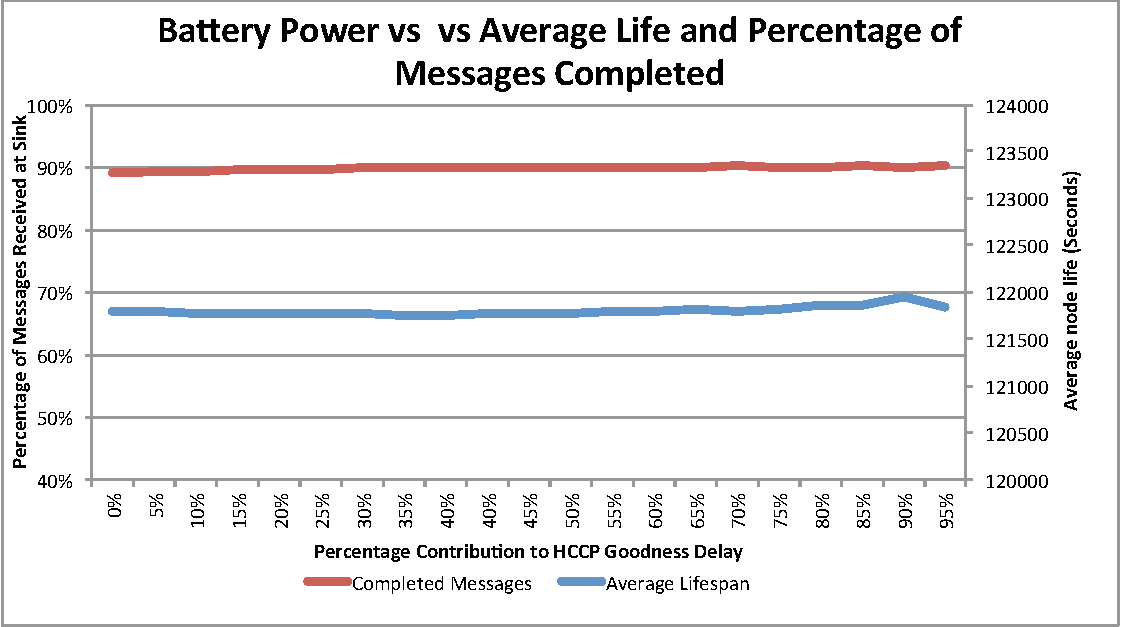
\includegraphics[width=0.9\textwidth]{images/simulation/goodness/Battery4.pdf}
	\caption{The relationship between HCCP Goodness Delay using Available Battery Power size and simulation results.}
	\label{fig:images_simulation_goodness_Battery2}
\end{figure}


An interesting result of focusing on Battery Power is that fewer messages are lost
due to motes dying. This makes sense, since as the battery in the mote nears depletion, 
the mote will not elect to be a clusterhead. Because the mote is not a clusterhead, the 
mote is not accepting messages from surrounding motes, rather it is getting rid of 
all the messages in its message queue. Then, once the mote finally dies, its 
message queue will be as empty as possible and minimal messages are lost.  

This
effect can be see in in Figure~\ref{fig:images_simulation_BatteryVsLeach_Death}.
The election protocol in LEACH is naive, electing clusterheads at random, causing
motes that are nearing death to become clusterheads. Notice that there is a 
high variability in how many messages are lost in dying motes in LEACH. 
In fact, the simulation results showed that there were motes that
died with their message queues completely full. HCCP, on the other hand,
has very low variability due to the network avoiding using dying motes as clusterheads.

The end result of using Battery Power as an HCCP factor, is that fewer messages are lost, 
therefore more messages successfully reach the sink. This can be seen in 
Figure~\ref{fig:images_simulation_BatteryVsLeach_Messages}.

\begin{figure}[htbp]
    \centering
        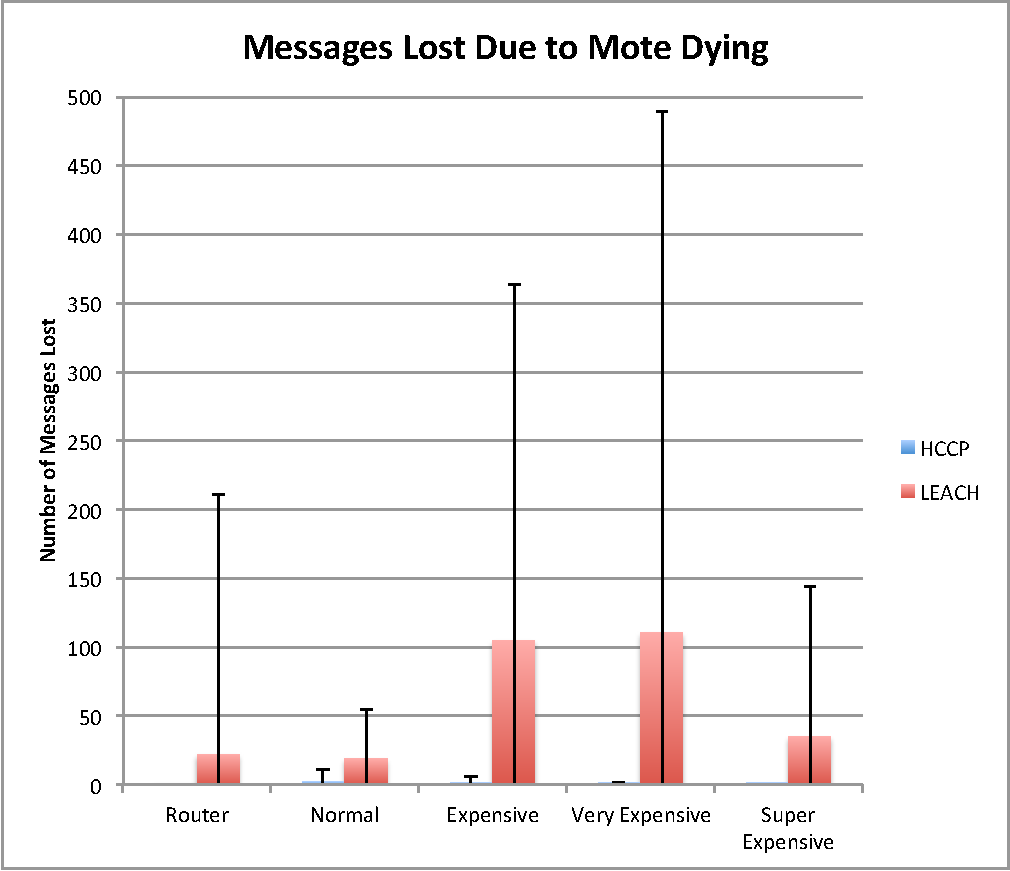
\includegraphics[height=3.75in]{images/simulation/BatteryVsLeach/Death.pdf}
    \caption{HCCP focused on Battery Power loses less messages since dying motes will not elect to be clusterheads.}
    \label{fig:images_simulation_BatteryVsLeach_Death}
\end{figure}

% from /Users/robg/charts/BatteryVsRandom4-noSinkSleep/
\begin{figure}[htbp]
    \centering
        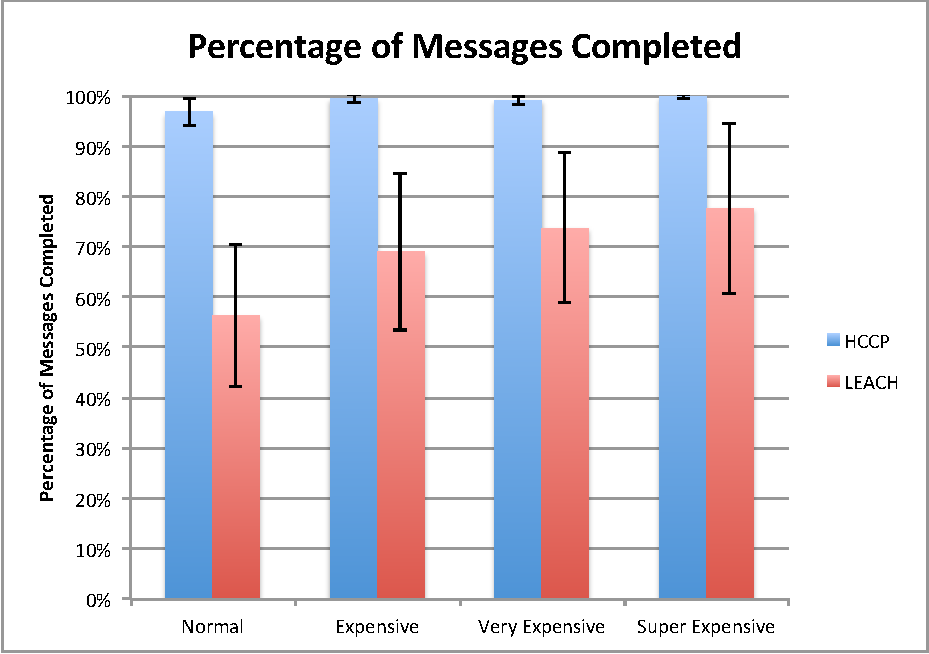
\includegraphics[height=3in]{images/simulation/BatteryVsLeach/Messages.pdf}
    \caption{HCCP focused on Battery Power has better throughput than LEACH since fewer messages are lost in dying motes.}
    \label{fig:images_simulation_BatteryVsLeach_Messages}
\end{figure}



\subsubsection{Effect of Duty Cycling on HCCP Goodness Delay}

\begin{figure}[htbp]
	\centering
		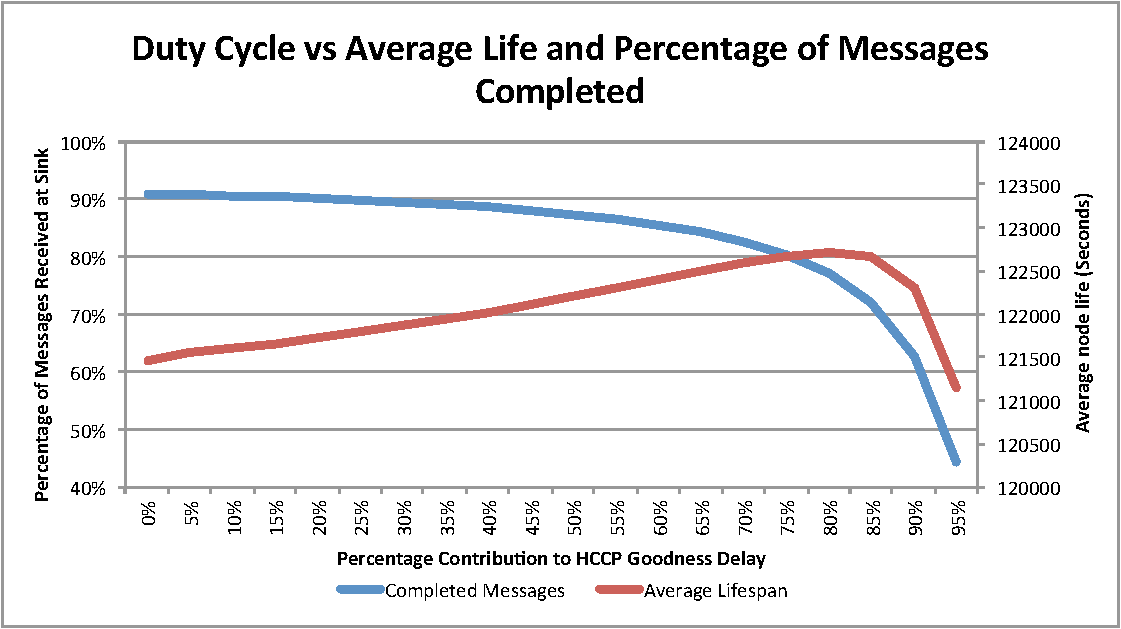
\includegraphics[width=0.9\textwidth]{images/simulation/goodness/Duty2.pdf}
	\caption{Visualization showing the relationship between HCCP Goodness Delay using Duty Cycling and simulation results.}
	\label{fig:images_simulation_goodness_Duty}
\end{figure}

The HCCP Duty Cycle factor causes motes to live longer, but deliver fewer messages. This is the
common WSN throughput versus lifespan tradeoff. As motes focus on duty-cycling, they 
become clusterhead less frequently, which causes message throughput to drop. This 
relationship can be seen in Figure~\ref{fig:images_simulation_goodness_Duty}, as 
the focus on Duty Cycling increases, the message throughput drops while the average mote lifespan 
increases. This trend is followed until 85\% focus on Duty Cycling, at which time the same effect as 
clusterhead percentage in LEACH occurs, too few motes are announcing themselves as clusterheads, causing 
the rest of the motes to be powered up longer waiting for clusterhead candidacy and clusterhead announcement messages.
Since these motes are on longer waiting for announcement messages, the lifespan drops. Though there are obvious 
gains for life span to focusing on Duty Cycling, Duty Cycling is a better secondary HCCP Goodness factor with a 
minority of the control of the Goodness Delay time.

The problem with Duty Cycle as the main HCCP Goodness factor is that it is not 
providing enough value to make up for the overhead that HCCP puts on the network.
At no time did HCCP using Duty Cycling beat LEACH in simulation. LEACH
has duty cycling built in to the design. HCCP uses that same duty cycling when 
choosing if the node should be a clusterhead, then describes how good the
clusterhead is by announcing the clusterhead sooner or later. HCCP Duty cycling doesn't 
add this value to the network, it only delays motes longer from announcing their Clusterhead
Candidacy if the mote has been a clusterhead recently. Using Duty Cycling in an HCCP 
Goodness Delay is therefore useless and should not be used because it costs more to run this
redundant idea than the benefit it provides to the network.




\subsubsection{Effect of Random Delay on HCCP Goodness Delay}
\label{randomDelay}


Randomness is the backbone of LEACH, in that each node creates a random number
to decide whether or not it should be a clusterhead. This factor in
HCCP's heterogeneous election is just a random number that will decide how long the
mote will delay before transmitting its candidacy message or clusterhead announcement. 
Using only the Random HCCP Goodness factor, HCCP degrades to a slightly mutated form of LEACH, as LEACH
draws a random number that decides how long the mote will delay before announcing itself as a clusterhead. HCCP takes this
idea, making the moderate change that motes will delay the random amount of time until it either
hears a better mote (better being defined as a mote that transmits its clusterhead candidacy earlier), or gets to 
transmit its candidacy message. 

\begin{figure}[tbhp]
	\centering
		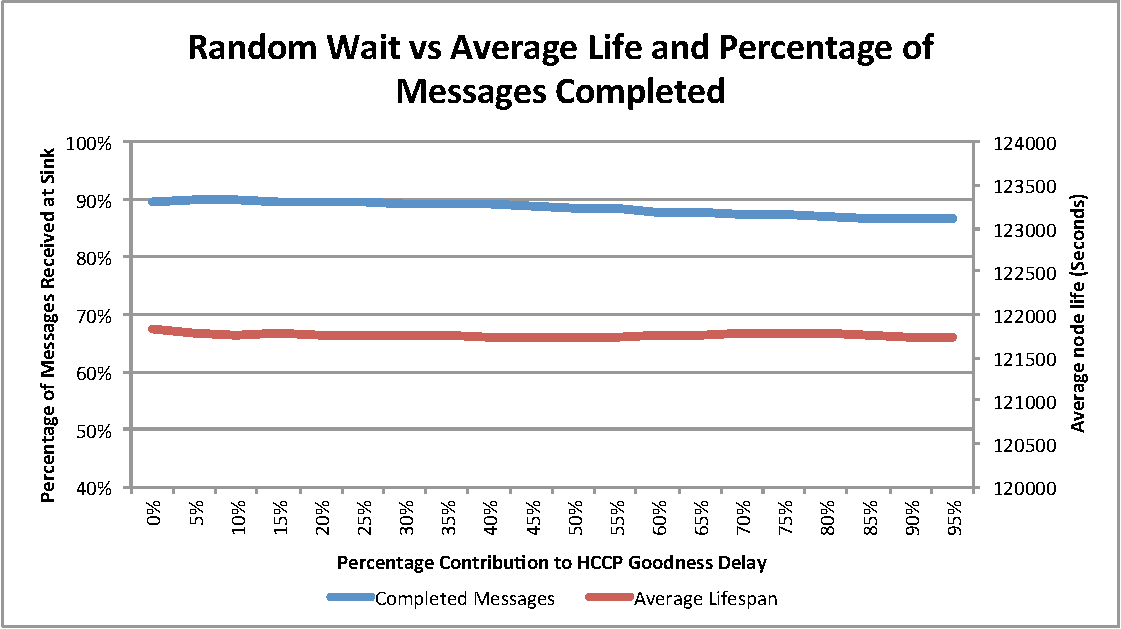
\includegraphics[width=0.9\textwidth]{images/simulation/goodness/Random3.pdf}
	\caption{The relationship between HCCP Goodness Delay using Random Wait Times and simulation results.}
	\label{fig:images_simulation_goodness_Random}
\end{figure}


Using Random as the
sole HCCP Goodness factor does not work well, as seen in Figure~\ref{fig:images_simulation_goodness_Random} Randomness
has very little effect on the network throughput or average node life. 
But Random works well paired with other factors 
as a tie-breaker, making one 
mote announce it's clusterhead status before a neighbouring node of similar
configuration. Using Randomness as a tie breaker works especially well early on in the
network's life, as many of the motes will have empty or nearly-empty messages queues and
full battery power. If two motes have the same Goodness Delay they will transmit their
candidacy or clusterhead announcement at the same time, potentially creating collisions
in the network.

\subsubsection{Effect of Sensor Mission on HCCP Goodness Delay}



Sensor mission is a percentage of how important the sensors are for a given mote. For instance,
a router mote with no sensors would have a sensor mission of 0\%, since it has no sensors. A
mote with very expensive sensors should almost never be a clusterhead, preserving its battery power
to collect more information. This value can be manually set, or automatically created by
counting the number of sensors that are being read and creating a Sensor Mission percentage from that
information.

\begin{figure}[tbhp]
	\centering
		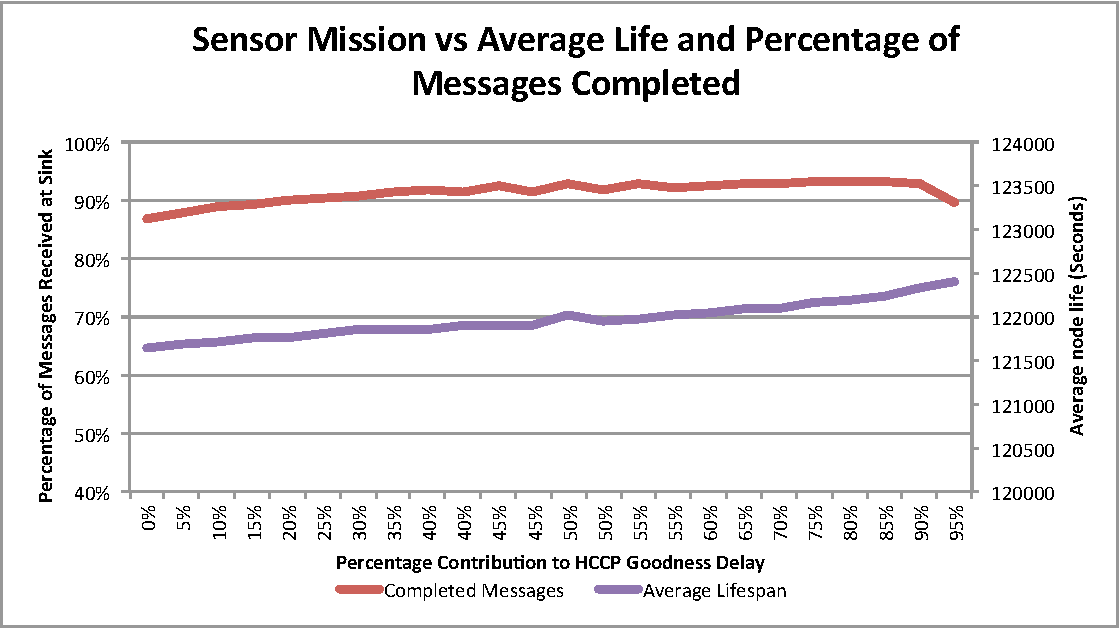
\includegraphics[width=0.9\textwidth]{images/simulation/goodness/Sensor2.pdf}
	\caption{The relationship between HCCP Goodness Delay using Sensor Mission and simulation results.}
	\label{fig:images_simulation_goodness_Sensor}
\end{figure}

Sensor mission creates a positive trend in both average node life and message throughput, as seen in 
Figure~\ref{fig:images_simulation_goodness_Sensor}. This
is because routers were given a sensor mission of 0 and sensor motes were given high Sensor Mission.
Providing motes with a Sensor Mission value is the best case as motes will then `know' how good
they are at the clusterhead task, making better router motes and motes with larger message queues
clusterhead motes more often. The problem with providing motes with Sensor Mission values is that
it is manual labour, and must be configured before the network is deployed. Also, Sensor Mission would 
be the most successful with a heterogeneous network; if all motes are the same and have the same Sensor
Mission, the clusterhead elections would degrade to an HCCP network that is 100\% focused on Random since all
motes would be generating the same Goodness Delay values.

%As discussed Section~\ref{simTuning}, he preset Sensor Mission is the ideal case for tuning a network to create long-lived
%networks. The results found in the simulation show that that preset Sensor Mission 

\subsubsection{Paired Factors in Heterogeneous Elections}
More than one factor can be paired together in the heterogeneous election to generate the Goodness
Delay. When networks first start, all message queues will be empty and all
batteries will be at 100\%, this will cause collisions during the 
HCCP Candidate Announcements, since all motes that elect to 
be a clusterhead that round will attempt to transmit their 
candidacy at about the same time (which will be close to immediately) if
the HCCP Goodness Delay is 100\% generated from a single factor. 
Adding a small percentage of the Random factor  will vary the 
generated transmission times, preventing the problem of equal Goodness Delays.

When adding Randomness to the Goodness Delay calculation will first
generate a goodness based on a primary factor (such as Available Message Queue Size or
Available Battery Power) which makes up the majority of the time, say 90\%. 
The Randomness will make a 10\% variance of the remaining time. 
The variance in the delay time will effectively be a tie-breaker for the transmission times
for the motes, avoiding many collisions while sending the announcements. The drawbacks to adding 
the Random factor to the Goodness Delay is that it adds no value to the Goodness Delay, as discussed
in Section~\ref{randomDelay}. Though, a small amount of Random Delay in the network 
is beneficial to the network due to the collisions it avoids. 


\subsection {Tuning HCCP for Power Efficiency}
\label{simTuning}
%lifespanCompare_higherfreq/comareLifespan.xlsx

\begin{figure}[htbp]
    \centering
        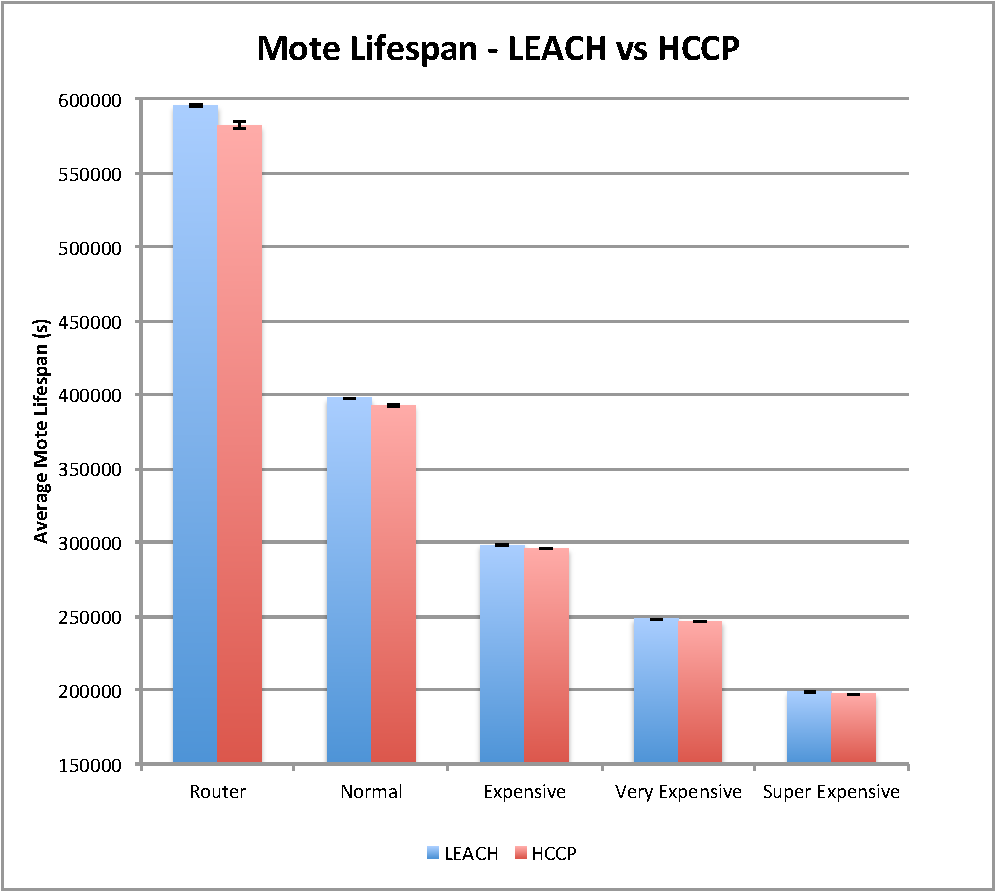
\includegraphics[height=3.5in]{images/lifespan/life.pdf}
    \caption{Tuning the efficiency of HCCP by minimizing Roundtable discussion allows HCCP to have networks lifespans approximately equal to LEACH.}
    \label{fig:images_lifespan_life}
\end{figure}

\begin{figure}[htbp]
    \centering
        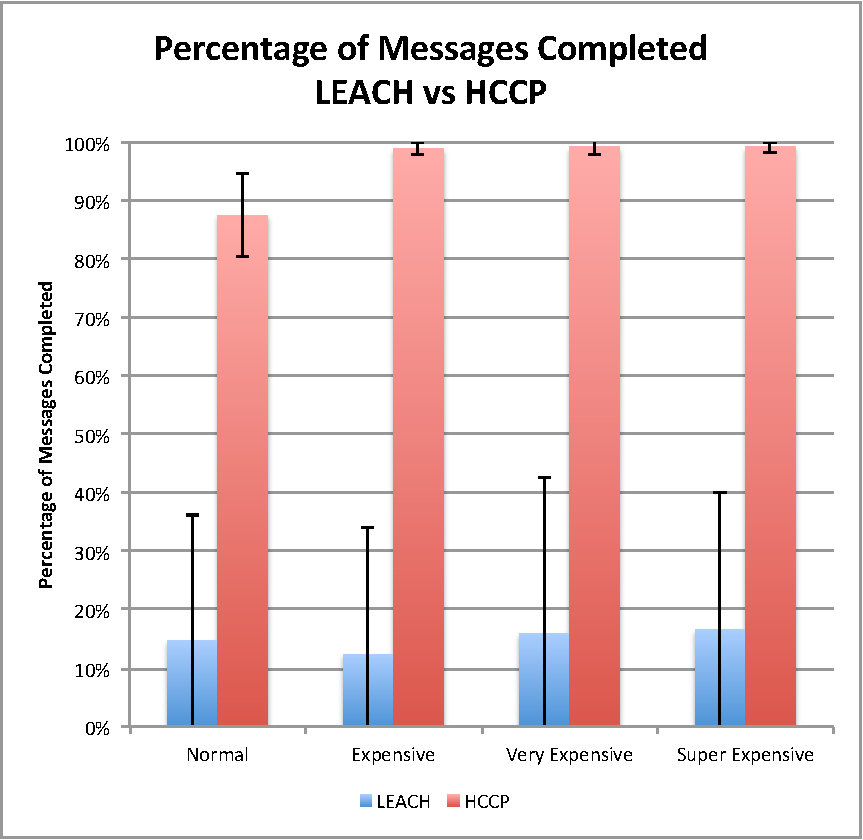
\includegraphics[height=3.5in]{images/lifespan/messages.pdf}
    \caption{In a tuned network, HCCP still has a much higher message throughput.}
    \label{fig:images_lifespan_messages}
\end{figure}

HCCP adds more time where all the motes are fully powered on than LEACH, because of the Roundtable Discussion 
and Clusterhead Candidacy stages. These extra steps cause an energy drain on the network,
but add lots of value to the network in terms of message throughput and data dissemination. 
As mentioned in Section~\ref{implementationTuning}, HCCP can be tweaked to be more power efficient while
still utilizing the gains from the Goodness Delay.

The easiest gain is to eliminate the Roundtable Discussion. This will improve network life, but decrease the 
ability to quickly disseminate information. For static networks that require a long lifespan, this is a good option.

The other option is to eliminate the Two-Stage Election, by eliminating the Clusterhead Candidacy stage. To compensate
for not having the Clusterhead Candidacy stage, the Clusterhead Election stage can be used to implement
the Goodness Delay features. To do this: in the Clusterhead Election, if a different mote announces itself
as a clusterhead first, concede being a clusterhead and become a clustermote. This is the same idea as used in Clusterhead Candidacy, but
done at the same time as a Clusterhead Election. The network will then choose slightly less optimal clusterheads, 
but overall creates a gain in which motes elect to be clusterheads. See Section~\ref{noCC} for more details about not using 
a Clusterhead Candidacy phase.

A well-tuned HCCP network will have a slightly shorter lifespan than a comparable LEACH network, but will have a
much higher message throughput than the LEACH network due to the quality of clusterheads that are chosen.
If lifespan is more desirable than message throughput, the Sleep period between 
election cycles could be extended to add lifespan to the network, which would make HCCP have a longer
lifespan for the same message throughput as LEACH.

A simulation was created with the HCCP and LEACH phases set to the same length. The results can 
be seen in Figures~\ref{fig:images_lifespan_life} and \ref{fig:images_lifespan_messages}.
LEACH has a longer lifespan, but dismal message throughput, while HCCP has
excellent message throughput. The lifespan of the router mote is noticeably lower in 
HCCP due to HCCP leveraging the router motes to be clusterheads more frequently, which 
in turn is increasing the message throughput. Consequently, the  router motes have 
shorter lifespans as the network relies on the routers to become clusterheads more frequently. 




\subsubsection{Eliminating the Clusterhead Candidacy Phase}
\label{noCC}
The Clusterhead Candidacy phase is a phase in HCCP that can be considered overhead, and 
is an obvious target to eliminate when looking to achieve longer lifespans. The Clusterhead
Candidacy phase offers very little in the way of overhead, however, since all motes that are not considering
being a clusterhead are sleeping during this phase. The clusterhead motes will then 
have time to share information about which motes should be clusterheads for that round. If the
Clusterhead Candidacy phase is dropped, the functionality must be moved to the Clusterhead Election phase.

The new Clusterhead Election phase would then work as follows: 
\begin{enumerate}
    \item Choose to be a clusterhead or not
    \item Listen for clusterhead elections. If clusterhead, use Goodness Delay to discover how long to wait until it is time to Announce itself as clusterhead.
    \begin{itemize}
        \item If a mote that has elected to be a clusterhead hears a clusterhead announcement before it sends one, choose to not be a clusterhead, and follow the mote that sent the clusterhead election.
    \end{itemize}
\end{enumerate}

%compareCCandNo_crazyHighFreq

\begin{figure}[htbp]
    \centering
        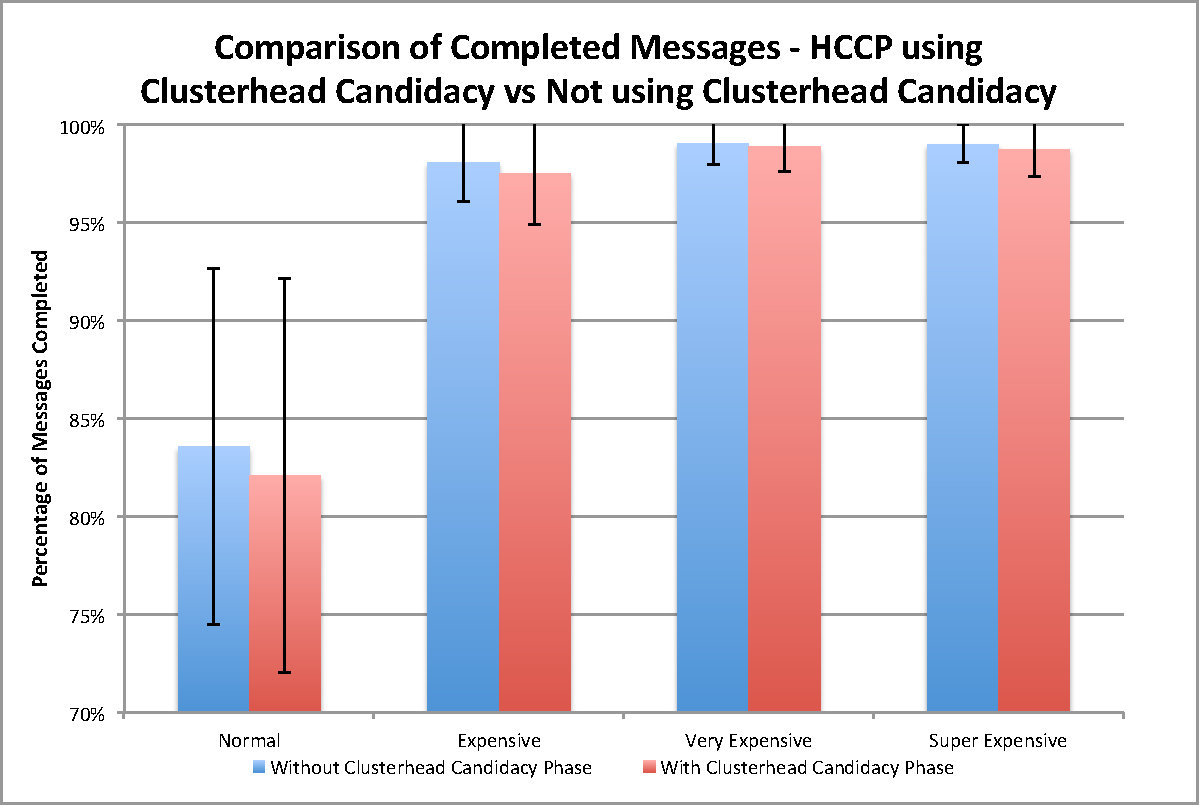
\includegraphics[height=2.9in]{images/ccVsNo/messages.pdf}
    \caption{ HCCP using Clusterhead Candidacy vs Not using Clusterhead Candidacy. The message throughput is comparable between the two networks.}
    \label{fig:images_ccVsNo_messages}
\end{figure}
\begin{figure}[htbp]
    \centering
        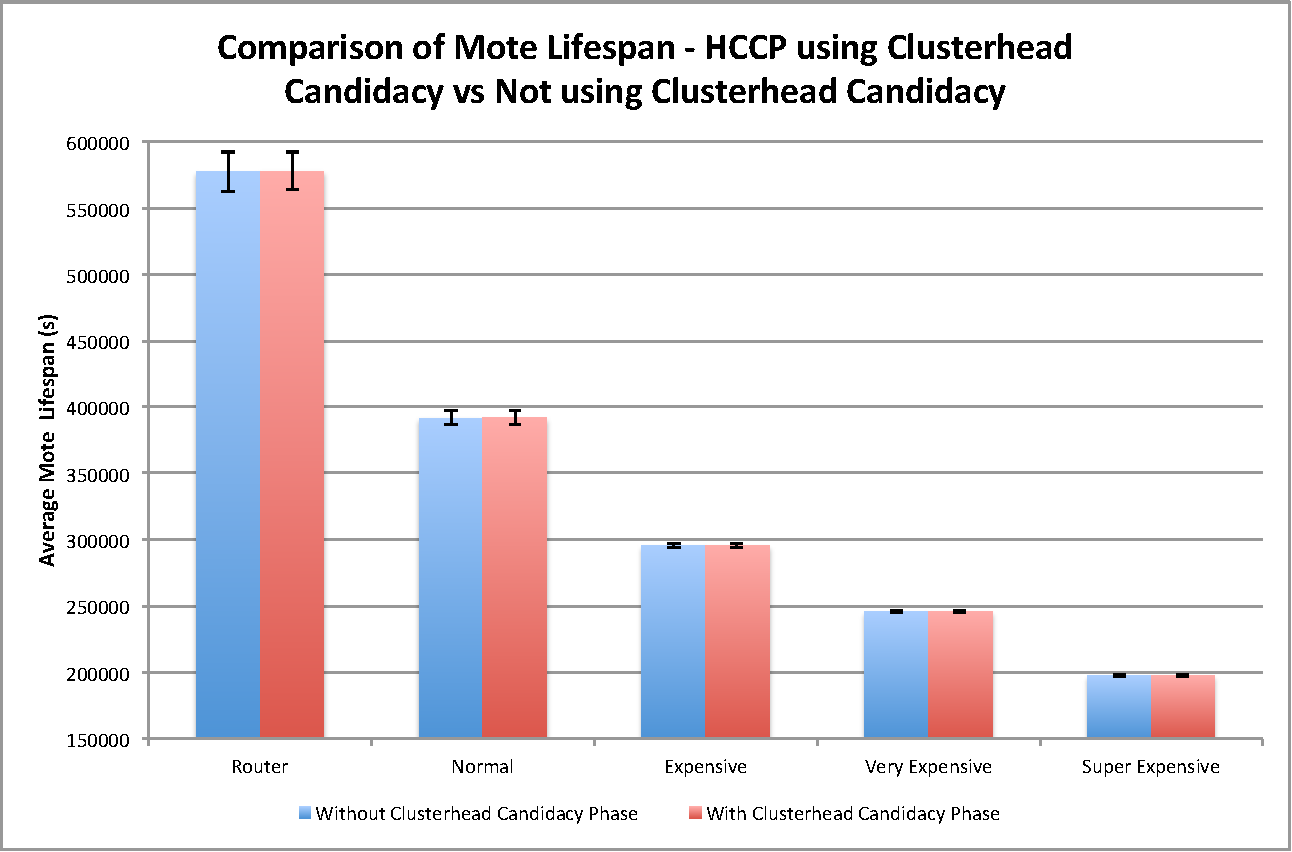
\includegraphics[height=3.1in]{images/ccVsNo/lifespan.pdf}
    \caption{HCCP using Clusterhead Candidacy vs Not using Clusterhead Candidacy. The results are quite even in terms of mote lifespan.}
    \label{fig:images_ccVsNo_lifespan}
\end{figure}


The rest of the protocol runs as previously prescribed. The problem with overloading the Clusterhead Announcement is that when
a collision occurs, it will cause much more damage to the entire cycle of the protocol. If a collision occurs during the 
Clusterhead Candidacy phase, one or both of the motes that are announcing their candidacy will opt to not be clusterheads, 
meaning that there will not be many collisions during the Clusterhead Announcement phase. When a collision happens in the
overloaded Clusterhead Announcement none of the motes in the neighbourhood will be able to follow either of the
motes that made the announcements, since the messages will be garbled. This means that the motes will continue listening for
clusterhead announcement messages, which means that these motes will at best be using the third best clusterhead mote in the neighbourhood (the next best
mote after the two motes that had a collision).

Two simulations were created with all parameters the same, with the exception that one of the simulations 
used a modified version of HCCP that dropped the Clusterhead Candidacy phase. The results, as seen
in Figures~\ref{fig:images_ccVsNo_lifespan} and \ref{fig:images_ccVsNo_messages}, show that whether the Clusterhead
Candidacy phase is independent, or merged into the Clusterhead Election phase the results are approximately 
the same. This means that though merging the Clusterhead Candidacy and Clusterhead Announcement phases saves
energy since motes are not on as long each cycle, clustermotes are using poorer clusterheads each round.
Based on the simulation results, 
there is very little difference between running HCCP in either of these configurations, so either could be used in 
a physical deployment. 




\subsubsection{Sink Sleep vs Suboptimal Clusterheads}

The HCCP Clusterhead Candidacy stage causes an issue called HCCP Blocking (previously discussed in 
Section~\ref{hccp_blocking}) where messages will not flow into 
motes that are in range of the sink. There are two methods of allowing messages to get into the
motes that are in radio range of the sink:
\begin{itemize}
    \item allow the sink to sleep some percentage of the time, or
    \item have suboptimal clusterheads which will elect to be clusterhead despite the fact there is a better clusterhead in the neighbourhood. 
\end{itemize}
There are drawbacks to both of these options. If the sink is asleep, no messages are being received at the sink, which could effect how
many messages reach the sink. If suboptimal clusterheads are used, more motes are electing to 
be clusterheads, more motes are clusterheads, which puts a larger drain on more motes.

Simulations were run to see which method is better for solving the HCCP Blocking problem. 
Simulations were run with 20 repetitions each, using the same starting seeds. 
Figure~\ref{fig:images_SleepVsNo_Messages} shows that there were no real differences with 
the percentage of messages received at the sink. This means that even if the sink sleeps
every few rounds, there is no effect to the throughput of the network. This makes 
sense, as messages must flow into the motes adjacent to the sink before they can be 
hopped into the sink. Whether the sink sleeps, or motes elect to be 
suboptimal clusterheads, the path taken will be approximately the same. Note that 
router motes in the simulation did not make messages, and are therefore left off the chart.

There is also a concern that if the suboptimal clusterhead option is chosen, then 
the lifespan of the network might be lessened, since more motes will be clusterheads
at the same time. Figure~\ref{fig:images_SleepVsNo_MoteLife} shows us that 
the there is no significant hit to the network life. While difficult to see in the chart, there 
is no statistical difference between the two options for the `Super Expensive' motes 
(196734 $\pm$ 611 for Sink Sleep Super Expensive motes, 196782 $\pm$ 624 for Suboptimal
Super Expensive motes). 
%Data from Charts/SleepVsNo

There were also no significant differences between the two methods in terms of 
number of collisions in the network. This is also interesting since 
suboptimal clusterheads means that there will be more traffic in more areas, clusterheads
will be closer to one another.

\label{sleepVSsubop}
\begin{figure}[htbp]
    \centering
        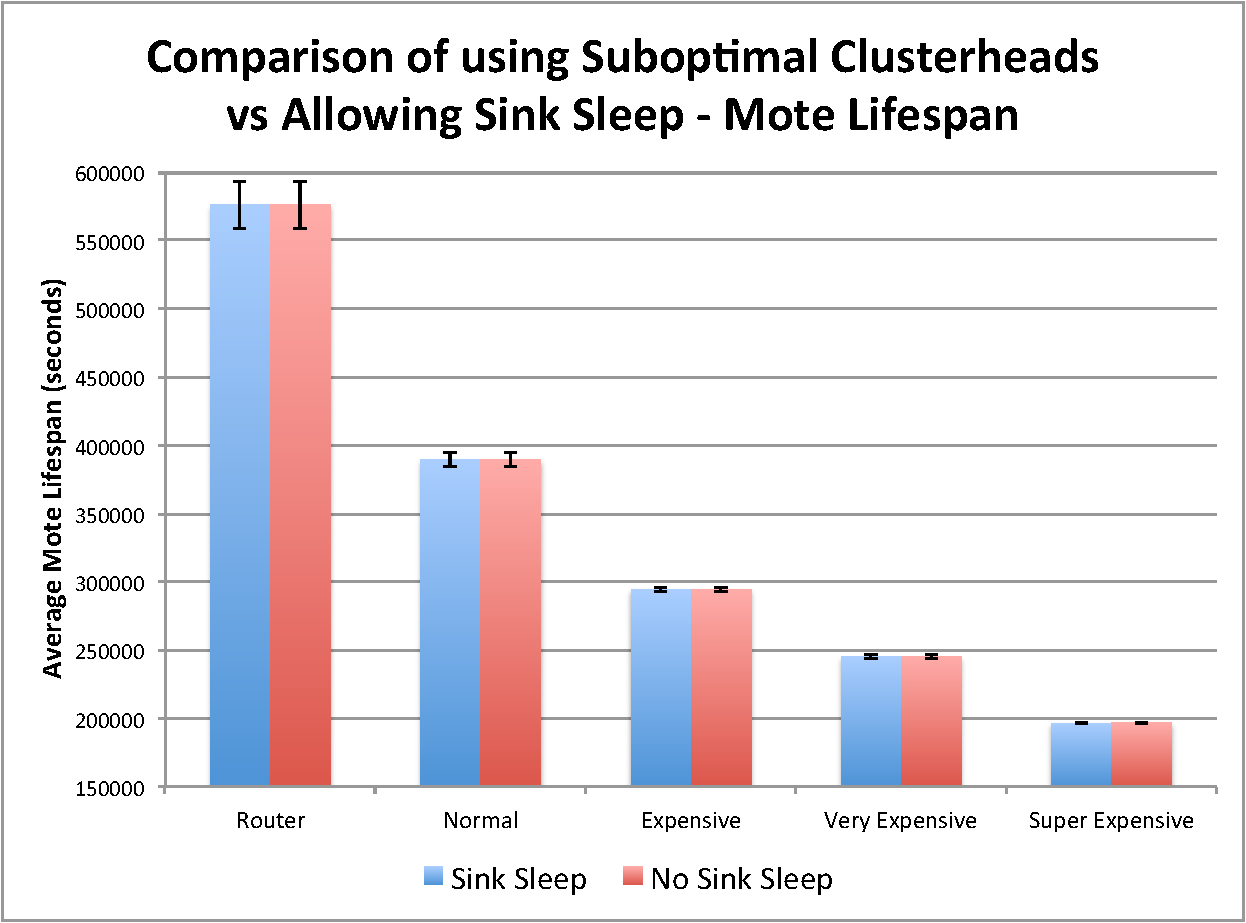
\includegraphics[height=3.2in]{images/SleepVsNo/Messages.pdf}
    \caption{The percentage of messages created that were received at the sink is approximately the same whether the sink periodically sleeps or not.}
    \label{fig:images_SleepVsNo_Messages}
\end{figure}

\begin{figure}[htbp]
    \centering
        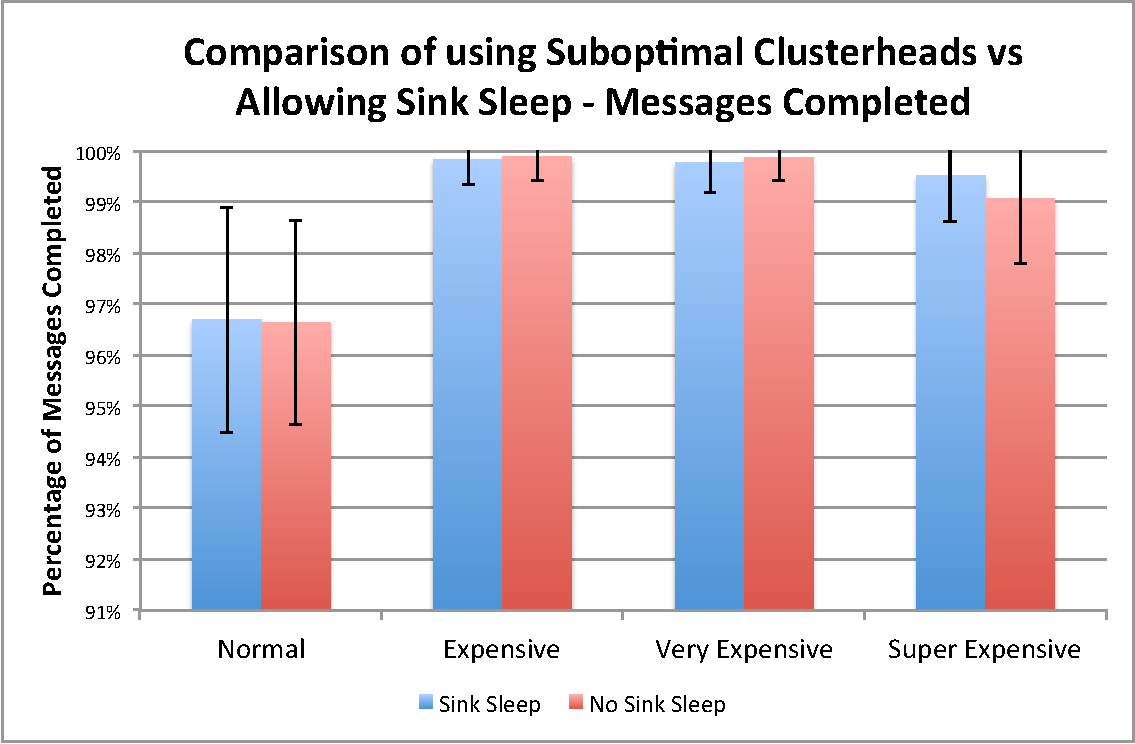
\includegraphics[height=3.2in]{images/SleepVsNo/MoteLife.pdf}
    \caption{Average mote lifespan is unaffected by whether the sink periodically sleeps or not.}
    \label{fig:images_SleepVsNo_MoteLife}
\end{figure}

\subsubsection{Clusterhead Opt-out}
As discussed in Section~\ref{optout}, if a network is set up to do multiple iterations of 
the TDMA schedule, clusterheads should be able to opt out during the Roundtable 
Discussion.
After running some test simulations to show that this could be a successful 
idea, contradictions in the concept were found which showed how the idea is 
flawed.
To successfully have a long-lived network, the Roundtable Discussion 
should be as short as possible, or left out altogether as the whole
network must be on for the stage to be fully utilized. Since Clusterhead Opt-out
requires Roundtable Discussion, its not a good fit for long-lived networks. In
general, it would be better to have one longer TDMA run schedule than a
repeated TDMA schedule. A longer TDMA schedule run allows the network to send as many 
messages as possible, and even allows motes to turn off when they are out of messages, and turn
back on and send more (provided it is still the mote's TDMA timeslice and the mote has
more messages ready to send).
Conversely, repeated TDMA schedules keep the same clusterhead, putting a large
load onto one clusterhead and losing a large amount of network adaptivity. Another 
drawback is throughput. Since one mote remains a clusterhead for an extended period of time, 
it can't send the messages it's collecting to motes closer to the sink. This causes the
messages are hopped much slower, causing message queues to fill.

There are instances where  Clusterhead Opt-out could still be useful, such as
networks that require quite long lifespans, where motes may go temporarily offline
or die at a frequent rate. The one election with many TDMA schedules would
allow the motes to send in their readings if and when they can. If one large
TMDA schedule is run and missed, motes will not be able to send in their readings
since they may be dead by the time the next large TDMA schedule is published.
This is, unfortunately, quite difficult to show in simulation, but presented 
as a possible niche case where Clusterhead Opt-out could still be useful.


\subsubsection{Automated Ad Hoc Backbone with HCCP}
There has been research into two-tier networks and networks with a backbone set of motes that are
set in the network for routing messages. LEACH does not take advantage of 
the benefits offered by these motes, as it does not consider the heterogeneity in the network. Heinzelman et al.~\cite{leach}
mention that a two-tier network could be created where the routing motes collect from the neighbourhood motes,
then run a LEACH schedule across the routing motes where \emph{only} the 
routing motes handle routing the messages to the sink.
The problem that exists with this model is that if the backbone gets broken,
there is no way for the network to recover, as shown in Figure~\ref{fig:images_BrokenBackbone_Backbone} (note that the sink is 
not visible in the figure). 
No motes past the break in the backbone will be
be able to send messages to the sink.

\begin{figure}[tbp]
    \centering
        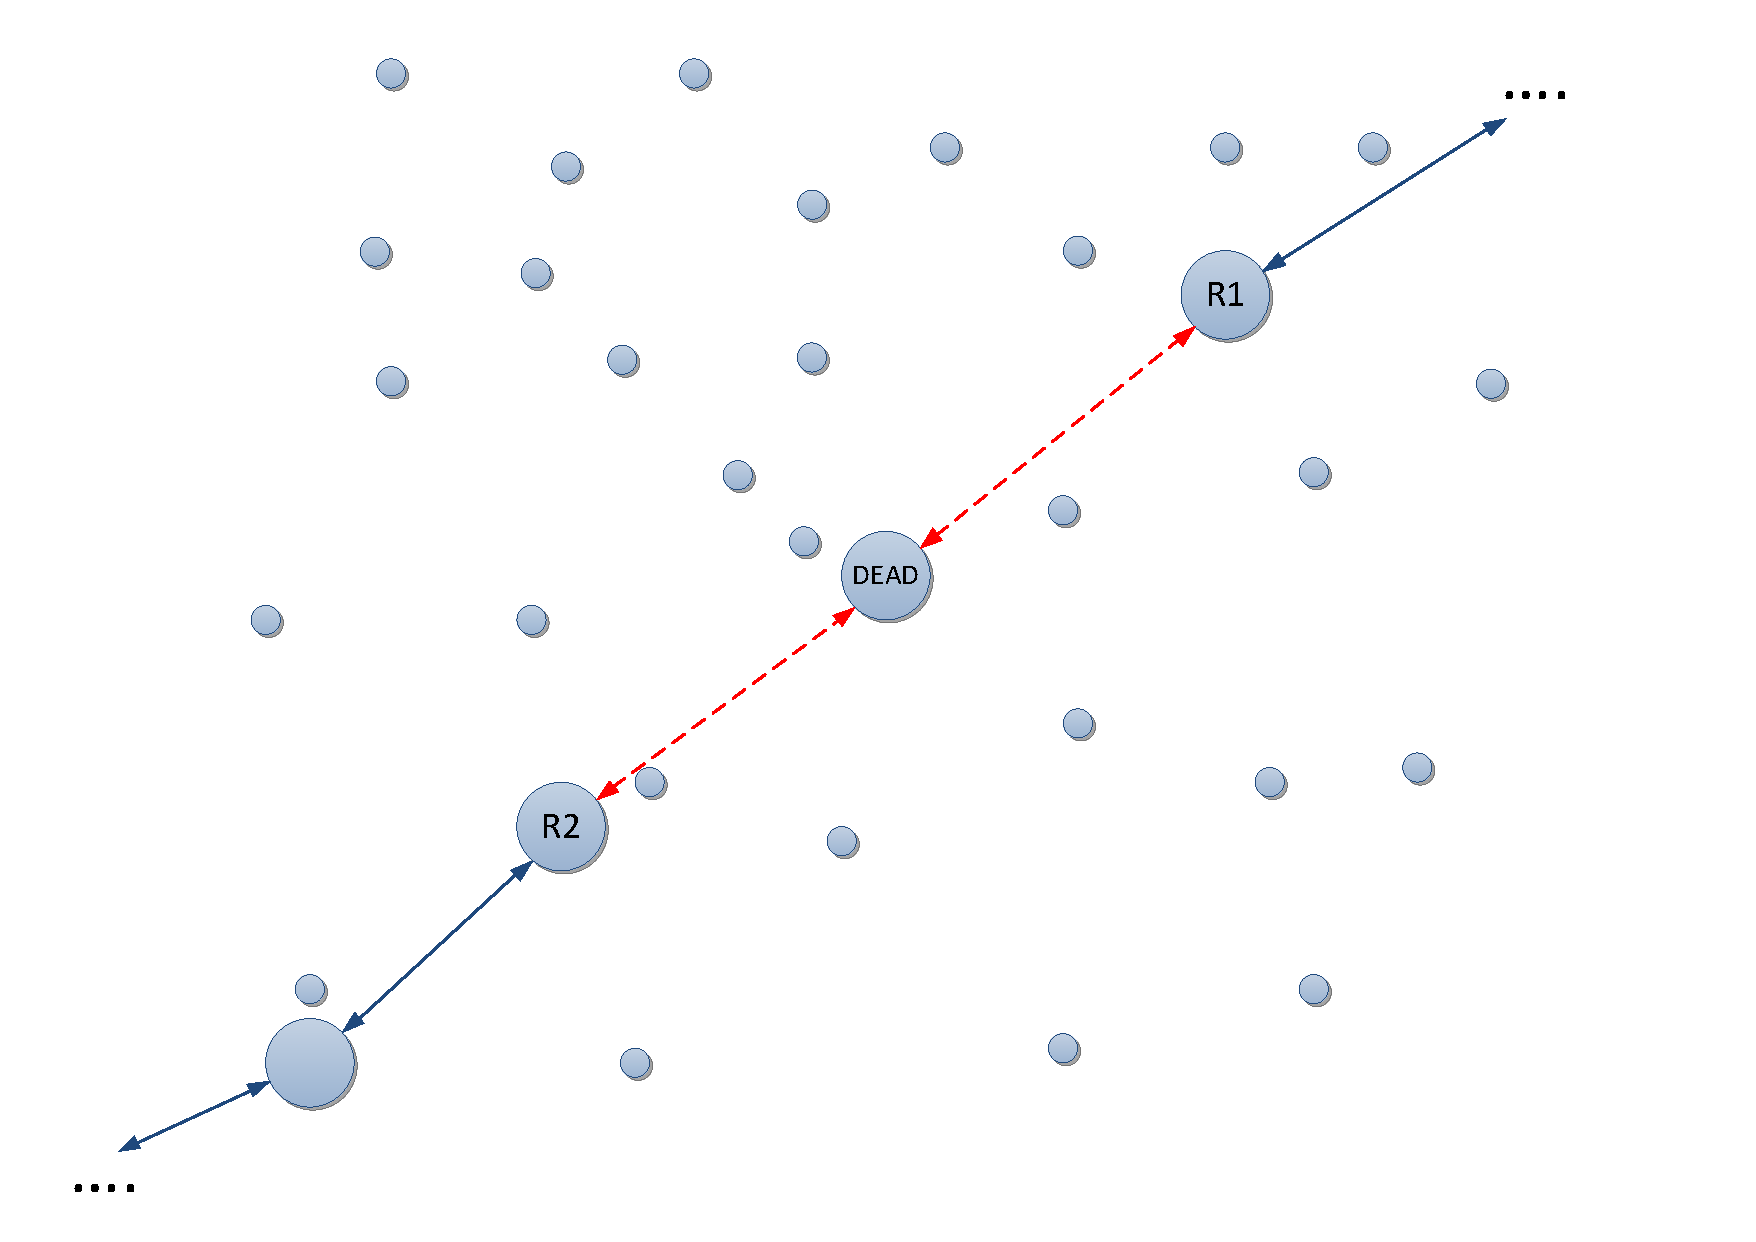
\includegraphics[width=6.5in]{images/BrokenBackbone/Backbone.pdf}
    \caption{Snapshot of a part of a WSN: routing mote R1 can not communicate with routing mote R2 because the routing backbone is broken.}
    \label{fig:images_BrokenBackbone_Backbone}
\end{figure}


HCCP uses LEACH as a starting point, but eliminates this problem by 
distributing the clusterhead task to all motes in the network. HCCP will ensure that
motes which are better at the clusterhead task will choose to be a clusterhead more often 
than motes which are not as good at the clusterhead task. This is due to the Goodness Delay that
is part of the clusterhead election. Motes with larger message queues, or more battery power,
or that have been given a low Sensor Mission value will choose to be clusterhead motes more often.
Due to this, motes that are not good clusterheads will not choose to be clusterheads,
and motes that are good clusterheads will choose to be clusterheads. This will create an 
ad hoc backbone across the motes which are inclined to be clusterheads. But, if the backbone is broken
by a mote dying or going offline, the messages from beyond the break can still move past the break. This
is because all motes can assume the clusterhead role. If there is no router mote in an area (due to the 
router mote going offline, or poor network distribution), other motes in the network will take on the 
clusterhead role. This will cause the motes that are non-router motes to die sooner, but 
keep the messages from the network flowing through areas with no router motes.

The HCCP Goodness Delay creates more robust networks that can 
handle change within the network with minimal negative effects to 
the network. Messages will still be routed well due to the 
Roundtable Discussion sharing routing information, and 
messages can move  over breaks in backbones since all motes can be assigned the clusterhead task.


%\textbf{Implement `failing' as a clusterhead. HCCP will recover, LEACH will not. -- add if there is time}
%This will need repeated schedules to work well. The runtime is now runtime/NumRepeats to keep the leach/hccp comparison 
%pretty consistent.
%\textbf{Movement... ugh. This would put the silver bullet in LEACH, but is hard to approach. - add if there is time}

